\section{Absorption, fluorescence and phosphorescence}
\label[section]{sec:AbsEmiFlourPhos}

The following section gives a brief introduction to principles important for spectroscopy.

Spectroscopy is the study of the interaction between electromagnetic radiation and matter. By examining the interaction of radiation with matter, spectroscopy provides valuable information about the composition, structure, and properties of substances. The basic principle of spectroscopy involves the effects such as absorption, emission, scattering and many more. In our case, the electronic transitions, therefore, absorption and emission are going to be the dominant processes.
\begin{figure}[h]
    \centering
    \begin{subfigure}[b]{0.3\textwidth}
        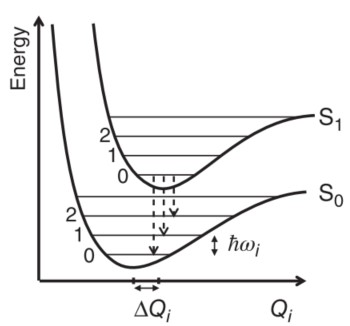
\includegraphics[width =\textwidth]{Bilder/Grundlagen/ElectronTransS0S1.jpg}      
        \caption{Curves of potential energy of a molecule as a function of the displacement from \cite{Kohler.2015}}
      \label{fig:S0S1}
    \end{subfigure}
    \hspace{0.03\textwidth}
    \begin{subfigure}[b]{0.65\textwidth}
      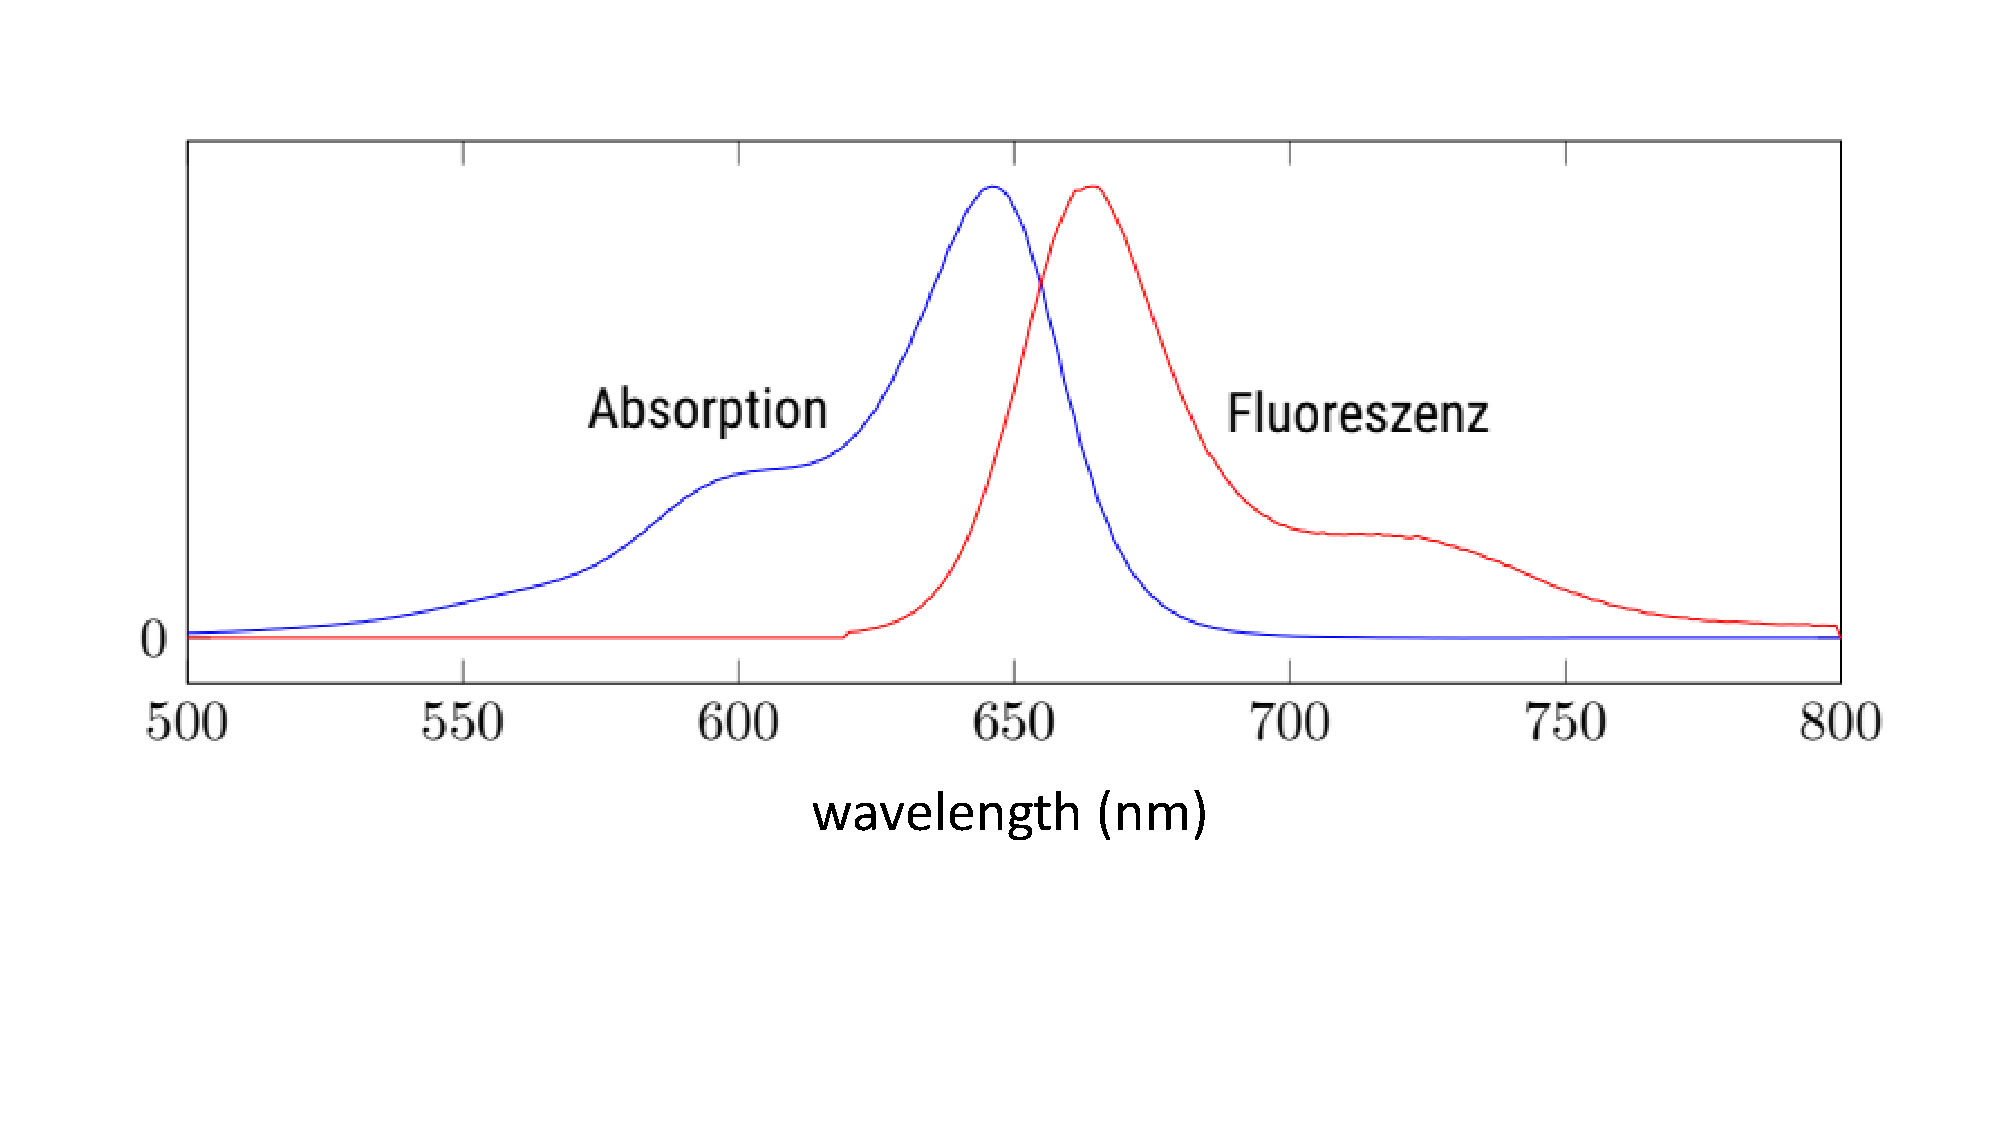
\includegraphics[width = \textwidth]{Bilder/Grundlagen/EmssionAbs_cropped.pdf}      
      \caption{Absorption and fluorescence spectrum of the dye BODIPY from \url{thermofischer.de}}
      \label{fig:AbsEmi}
    \end{subfigure}
    \caption{As depicted in (a), the emitted electrons cause ideally a mirror image of the absorption, as depicted in (b).}
    \label{fig:TheoAbsEmi}
\end{figure}

For pedagogical reasons, the effect of transitions is first introduced for singlet state transitions. In a single molecule, the quantum states $\ket{\Psi_{initial}}$ and $\ket{\Psi_{final}}$ are orthogonal. This leads to a transition dipole moment $M$ of 0 for the classical Hamiltonian. When introducing a perturbation in the case of a weak perturbation, the orthogonality of those two states is lifted. The electromagnetic perturbation in our case couples the two states and the transition dipole moment (TDM) are nonzero. It is important to note the TDI for emission and absorption are the same as $M$ is an observable and therefore a real number and
\begin{equation}
    \bra*{\Psi_{initial}}\hat\mu\ket*{\Psi_{final}} = M_{if} = M_{fi} = \bra*{\Psi_{final}}\hat\mu\ket*{\Psi_{initial}}
\end{equation}
is symmetric.

During absorption, a photon is absorbed with an energy corresponding to the transition. This leads to an 
absorption pattern that reflects the structure of the energy levels of an atom as depicted in \cref*{fig:TheoAbsEmi}.

After absorption, the electron relaxes into the ground state from the excited state. This is called \textit{Kasha's rule}. From then on, it can perform either a radiative or a non-radiative transition to the ground state. Furthermore, it is possible to perform a transfer to a triplet state if the energy gap is very small. These processes tend to happen rarely, as the spin has to be flipped. This usually implies strong spin-orbit coupling. The radiative transition from a triplet state to the ground state is called \textit{phosphorescence}.




